\documentclass[11pt]{amsart}


\usepackage[ibidtracker=false,uniquename=false,giveninits=true,terseinits=true,backend=biber]{biblatex}
\usepackage{float}
\usepackage{graphicx}
\usepackage{todonotes}
\usepackage{subcaption}
\usepackage{amsmath}
\usepackage{amsthm}
\usepackage{amssymb}
\usepackage{algorithm}
\usepackage[noend]{algorithmic}
\usepackage[foot]{amsaddr}
\usepackage[misc]{ifsym}
\usepackage{enumitem}
\usepackage{geometry}
\usepackage[hidelinks]{hyperref}

\renewbibmacro{in:}{}
\addbibresource{rnni_geometry.bib}
\AtEveryBibitem{
	\clearlist{language}
}

\setlist{leftmargin = 0pt}
\geometry{margin=1in}


\newtheorem{proposition}{Proposition}
\newtheorem{theorem}{Theorem}
\newtheorem{lemma}{Lemma}
\newtheorem{corollary}{Corollary}
\newtheorem{problem}{Problem}
\newtheorem{conjecture}{Conjecture}

% \renewcommand{\theoremautorefname}{Theorem}

\newcommand{\tocite}{ {\color{red}\fbox{CITATION}} }
\newcommand{\rnni}{\mathrm{RNNI}}
\newcommand{\findpath}{\textsc{FindPath}}
\newcommand{\mrca}{\mathrm{mrca}}
\newcommand{\rank}{\mathrm{rank}}
\newcommand{\ntime}{\mathrm{time}}
\newcommand{\nni}{\mathrm{NNI}}
\newcommand{\spr}{\mathrm{SPR}}
\newcommand{\tbr}{\mathrm{TBR}}
\newcommand{\fp}{\mathrm{FP}}
\newcommand{\dtt}{\mathrm{DtT}}
\newcommand{\np}{\mathbf{NP}}
\newcommand{\decprob}[1]{\rnni(#1)\text{-}\mathrm{SP}}
\newcommand{\rad}{\mathit{rad}}
\renewcommand{\O}{\mathcal O}
\renewcommand{\epsilon}{\varepsilon}
\renewcommand{\thesubfigure}{\Alph{subfigure}}

\newcommand{\algorithmautorefname}{Algorithm}

\newcommand{\summary}[1]{\textbf{#1}} % Print summaries to .pdf
% \newcommand{\summary}[1]{} % Hide summaries in .pdf

\newcommand{\todefine}[1]{{\color{blue}{We need to define:#1}}} % Print summaries to .pdf

\DeclareMathOperator*{\argmin}{argmin}

\graphicspath{{figures/}}

\sloppy


\title[Geometry of ranked tree spaces]{The Geometry of the Ranked Nearest Neighbour Interchange Space}
\date{\today}
\author{Lena Collienne}
\email{lcollienne@cs.otago.ac.nz}
\address{Department of Computer Science, University of Otago, New Zealand}
\author{Alex Gavryushkin\textsuperscript{\Letter}}
\email{\textsuperscript{\Letter}alex@biods.org}
\thanks{}

\begin{document}

\begin{abstract}
\end{abstract}

\maketitle


\section{Introduction}

\summary{Why we want time-trees}

\summary{Why discrete time-trees -- Summarising for example}

\summary{How recent results about $\rnni$ make this space interesting and that it is strongly connected to $\dtt$}

\summary{Why we want to investigate geometrical properties of $\dtt$ and $\rnni$, and also $\rnni(\rho)$}

\summary{Structure of the paper.}


\section{Technical Introduction}

\summary{Introducing discrete time-trees and ranked trees}
A binary rooted phylogenetic tree is a binary tree on a fixed number $n$ of leaves, which are uniquely labelled by elements of the set $\{a_1, \ldots, a_n\}$.
The main objective of study in this paper, \emph{discrete time-trees}, are such binary rooted phylogenetic trees, where leaves are assigned time $0$, and internal nodes are uniquely assigned integer-valued times, such that an internal node always has time greater than its children.
We refer to the time of an internal node $v$ by $\ntime(v)$.
If not stated otherwise, we will refer to discrete time-trees simply as \emph{trees}.
The number of discrete time-trees with root time less or equal to $m$ is $\frac{(n-1)!n!m^{n-1}}{2^{n-1}}$ \autocite{Gavryushkin2018-ol}.
Discrete time-trees with root time $n-1$ are called \emph{ranked trees}, and we say \emph{rank} of $v$ to mean its time ($\rank(v) = \ntime(v)$) in a ranked tree to be consistent with notations used in \autocite{Collienne2020-iu}.
Two trees are \emph{identical} if there is a graph isomorphism between them preserving leaf labels and times.

Every internal node $v$ of a tree $T$ can be referred to by the set $C$ of leaves that are descending from this node.
We call such a set $C$ \emph{cluster} and say that the cluster $C$ is \emph{induced} by $v$.
A ranked tree can then be seen as a list of clusters $[C_1, \ldots, C_{n-1}]$, where cluster $C_i$ is induced by the internal node with time $i$ for $i \in \{1, \ldots, n-1\}$.
For each subset $S \subseteq \{a_1, \ldots, a_n\}$ we call the internal node of a tree $T$ with lowest time that is ancestral to all elements of $S$ the \emph{most recent common ancestor} of $S$ and denote it by $(S)_T$.
We denote the parent of a leaf $a_i$ in $T$ by $(a_i)_T$.

\summary{Defining the tree space $\dtt_m$ and $\rnni = \dtt_{n-1}$}
The main objective of this paper is to study the graph $\dtt_m$ of discrete time-trees, which is defined as follows.
The nodes of $\dtt_m$ are trees with root time less pr equal to $m$.
Trees $T$ and $R$ are connected by an edge if performing one of the following (reversible) operations on $T$ results in $R$:
\begin{enumerate}
	\item An \emph{$\nni$ move} connects trees $T$ and $R$ if there is an edge $e$ in $T$ and an edge $f$ in $R$, both of length one, such that shrinking $e$ and $f$ to nodes results in isomorphic trees.
	\item A \emph{rank move} on $T$ exchanges the times of two internal nodes, if the difference of their times is one.
	\item A \emph{length move} on $T$ changes the time of an internal node by one.
\end{enumerate}
\todo{Is this clear? Maybe using intervals (if we are going to define them)}
Note that length move can only change the time of a node in a tree $T$ if there is no node with this new time in $T$ already.
It is also important to see that our definition of $\dtt_m$ differs from the definition of \textcite{Gavryushkin2018-ol}, as length move are defined differently in their paper.
As natural definition, we consider distances between two trees $T$ and $R$ in this graph $\dtt_m$ to be the length of a shortest paths between these trees, and denote it by $d(T,R)$.

The ranked nearest neighbour interchange ($\rnni$) graph of \textcite{Collienne2020-iu} is the graph $\dtt_m$ for $m=n-1$, and hence is a graph of ranked trees.
Hence, length moves are not possible in this graph, and we use the notion $\rnni$ \emph{move} to mean either a rank move or an $\nni$ move.

\todefine{
	\begin{itemize}
		\item ??intervals, to make explanation of length move and how they are replaced in order to use FP easier??
		\item caterpillar path and shortest caterpillar path -> in caterpillar section
		\item convexity -> in caterpillar section
		\item representation of caterpillar trees as lists of leaves instead of cluster representation (?)
		\item $\rnni(\rho)$ -> in corresponding section
		\item rank interval for Lemma~\ref{lemma:nni_path_to_caterpillar} -> if we needed, in corresponding section
		\item cherry (for lemma~\ref{lemma:max_dist_ctree}) -> in caterpillar section (if needed)
		\item one-neighbourhood (for Theorem~\ref{thm:caterpillar_convex_rnni}) -> in corresponding section, if needed
	\end{itemize}
}


\section{Computing Shortest Paths in $\dtt$}

\todo{Do we want $\dtt$ or $\dtt_m$ in the titles of sections?}

\summary{Introduce how we can use $\findpath$ to compute $\dtt$ distances}
Distances between trees in $\rnni$ can be computed in quadratic running time with the algorithm $\findpath$, introduced by \textcite{Collienne2020-iu}.
As $\rnni$ is a special case of $\dtt_m$ for $m = n-1$, the question whether this algorithm can be generalised to compute distances in $\dtt_m$ arises.
Indeed, there is a way to use $\findpath$ to compute distances between trees in $\dtt_m$.
This works in two steps as it is briefly explained in the following, before we consider each of these steps in greater detail.
At first, leaves are added to both trees $T$ and $R$ in order to get two ranked trees $T_r$ and $R_r$ on with the same number of leaves.
Afterwards, we apply $\findpath$ to the pair of trees $T_r,R_r$, receiving the path $\fp(T_r,R_r)$.
With Theorem~\ref{thm:dtt_findpath} we see that this computes the distance $d(T,R)$ in $\dtt_m$ indeed.
To explain how ranked trees $T_r$ and $R_r$ can be received from adding leaves to trees $T$ and $R$, we assume that $T$ and $R$ are not ranked trees, as $\findpath$ could otherwise be applied to these trees directly.

\summary{How to add leaves to a $\dtt_m$ tree to transform it into a ranked tree}
Let $m$ to be the maximum time of the roots of $T$ and $R$.
To receive a ranked tree $T_r$ on $m+2$ leaves from $T$, we add leaves to $T$ as follows (\autoref{alg:ranked_tree}).
Note that the same can be done for $R$ to get a ranked tree $R_r$.
The root of $T_r$ is assigned time $m + 1$ and is connected to the root of $T$, such that one child of the root of $T_r$ is the subtree $T$.
\todo{Is this sentence sufficient to understand what's happening?}
The other subtree that is child of the root of $T_r$ is a caterpillar tree with leaves $\{a_{n+1}, a_{n+2}, \ldots, a_{m+2}\}$, such that $\ntime(a_{n+1}) = \ntime(a_{n+2}) < \ntime(a_{n+3}) < \ldots < \ntime(a_{m+2})$ and the resulting tree is a ranked tree with $m+2$ leaves.
An example of this extension of a tree $T$ to a ranked tree $T_r$ is depicted in \autoref{fig:dtt_to_ranked_tree}.

\begin{algorithm}[ht]
	\caption{RankedTree($T$)}
	\label{alg:ranked_tree}
	\begin{algorithmic}[1]
		\STATE $S:= \{1 \leq i \leq m | \text{ no internal node in } T \text{ has time } i\}$
		\STATE $[i_1, \ldots, i_{m-n+1}] = sort(S)$
		\STATE $T_r := T$ with additional internal node $v_1$ with children $a_{n+1}, a_{n+2}$ and time $i_1$
		\FOR {$k = 2, \dots, m-n+1$}
			\STATE Add internal node $v_k$ with with children $v_{k-1}$ and $a_{n+k+1}$ and time $i_k$ to $T_r$
		\STATE add internal node $\rho$ with children $v_{m-n}$ and $(\{a_1, \ldots, a_n\})_{T_r}$ to $T_r$
		\ENDFOR
		\RETURN $T_r$
	\end{algorithmic}
\end{algorithm}

\begin{figure}[ht]
	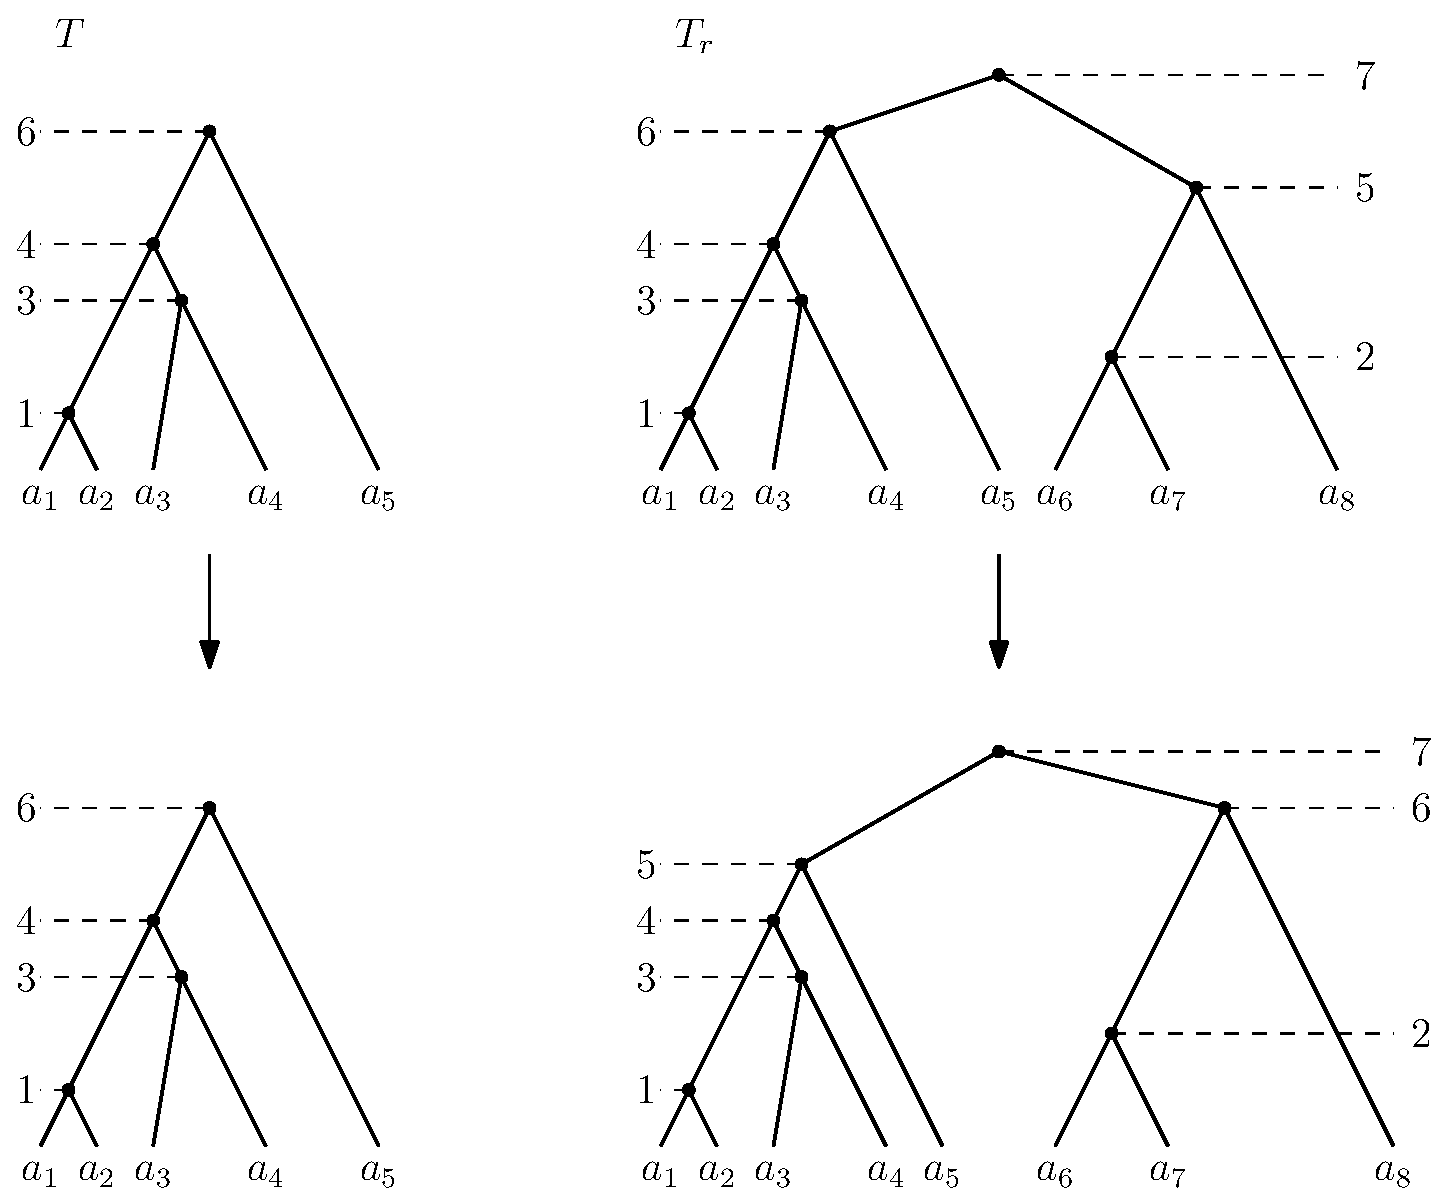
\includegraphics[width=0.75\textwidth]{dtt_to_ranked_tree.eps}
	\caption{Extending a tree $T$ on $n$ leaves in $\dtt_6$ (left) to a ranked tree with $m+2=8$ leaves (right) by adding a caterpillar subtree with three leaves.}
	\label{fig:dtt_to_ranked_tree}
\end{figure}

\summary{How to compute shortest $\dtt$-paths between trees with $\findpath$}
After extending both trees $T$ and $R$ to ranked trees $T_r$ and $R_r$ on $m+2$ leaves, $\findpath$ can compute a shortest path between $T_r$ and $R_r$ in the $\rnni$ graph on $m+2$ leaves.
As we know that $\findpath$ preserves clusters, there are no $\nni$ moves in the newly added caterpillar tree with leaves in $\{a_{n+1}, \ldots, a_{m+2}\}$ on $\findpath$.
Therefore, the only moves involving internal nodes of this caterpillar subtree are rank moves.
Each of these rank moves can be seen as a length move in the subtree that is rooted in $\{a_1, \ldots, a_n\}$, when ignoring the rest of the tree.
Hence the path $\fp(T_r,R_r)$ provides a path between $T$ and $R$, when only considering the subtrees induced by $\{a_1, \ldots, a_n\}$ in all trees on $\fp(T_r, R_r)$.
\todo{Do we want to use $\fp(T,R)$ for discrete time-trees $T$ and $R$?}
We denote this path in $\dtt_m$, which results from $\fp(T_r, R_r)$, by $\fp(T,R)$.
In \autoref{thm:dtt_findpath} we see that the $\fp(T,R)$ is a shortest path in $\dtt_m$ indeed.

\begin{theorem}
	The path $\fp(T,R)$ between two discrete time-trees $T$ and $R$ is a shortest path between these trees in $\dtt_m$, where $m$ is the maximum time of the root of $T$ and $R$.
	\label{thm:dtt_findpath}
\end{theorem}

\begin{proof}

\end{proof}

\summary{$\findpath$ distance in $\dtt$ is sum of $\fp(T,R)$ in $\rnni$ and length moves -- essential for later proofs}
With \autoref{thm:dtt_findpath} we can compute shortest path between two trees in $\dtt_m$ in polynomial time, more specifically in time $\O(m^2)$.
It furthermore follows that the distance between trees $T$ and $R$ in $\dtt_m$ is the sum of $\rnni$ moves and length moves on $\fp(T,R)$.

\begin{corollary}
	\todo{Do actually need this corollary?}
	Let $T$ and $R$ be discrete time-trees.
	Then the distance between $T$ and $R$ in $\dtt$ is:
	\[d(T,R) = r(T,R) + l(T,R),\]
	where $l(T,R)$ is the number of length moves, and $r(T,R)$ the number of rank and $\nni$ moves on $\fp(T,R)$.
\end{corollary}


\section{Geometrical Properties of $\dtt$}

\subsection{Caterpillar Trees}

\summary{The set of caterpillar trees is convex in $\rnni$.}
\begin{theorem}
	The set of caterpillar trees is convex in $\rnni$.
	\label{thm:caterpillar_convex_rnni}
\end{theorem}

\begin{proof}
	Let $T$ and $R$ be two caterpillar trees.
	For proving the lemma, we show that there is a tree caterpillar tree $T'$ in the one-neighbourhood of $T$ with distance $d(T',R) = d(T,R) - 1$ to $R$.
	The existence of a path between $T$ and $R$ that only consists of caterpillar trees then follows inductively.
	If there is a leaf that is part of the cherry in both trees $T$ and $R$, then the first tree on $\fp(T,R)$ is a caterpillar tree, which proves the statement.
	So we only need to consider the case that $T$ and $R$ have different cherries.
	Let $a_1$ and $a_2$ be the leaves of the cherry of $T$ and $a_3$ the leaf which has parent of rank two in $T$.
	Since neither $a_1$ nor $a_2$ are in the cherry of $R$, their parents must be different and therefore have different ranks in $R$.
	For the same reason, the parents of $a_1$ and $a_2$ also have a rank different to the parent of $a_3$ in $R$.
	% Two cases: $a_3$ above $a_1$ and $a_2$ in $R$ or one of $\{a_1,a_2\}$ is above $a_3$.
	\todo{Finish this proof!} 
\end{proof}

\summary{With Theorem~\ref{thm:caterpillar_convex_rnni} we can find a more efficient way to compute distances between caterpillar trees.}

\todo{Cite TSP paper -- caterpillar trees as special instance of TSP (lollipop graph)}

\begin{theorem}
	\todo{Do we want to use the represenation of caterpillar trees as sequence of leaves?}
	Let $T$ be an arbitrary caterpillar tree and $R$ the caterpillar tree $[1,2, \ldots, n]$.
	\todo{Note somewhere that we refer to the list representations of caterpillar trees by $T$, for example}
	Then it is
	\[d(T,R) = p_T - m_T,\]
	where $p_T$ is the number of transpositions in $T$ (Kendall-tau distance \tocite) and $m_T = |M_T|$ for
	\[{M_T} := \{i| (\forall k \text{ with } \rank(k)_T \leq \rank(i)_T: i < k) \text{ and } \rank(i)_T < \min\{\rank(1)_T, \rank(2)_T\}\}\]
	\todo{define the partial order $\preceq$}
	\label{thm:caterpillar_distance_formula}
\end{theorem}

\begin{proof}
	To prove the Theorem, we assume that $T$ and $R$ are caterpillar trees as described in the Theorem.
	We denote $\hat d(T,R) = p_T - m_T$ and prove $\hat d(T,R) = d(T,R)$.
	Similar to the proof of \autocite[Theorem 1]{Collienne2020-iu}, we only need to prove that for any caterpillar tree $T'$ in the one-neighbourhood of $T$ it is
	\begin{align}
		\hat d(T',R) \geq \hat d(T,R) - 1.
		\label{eq:distance_proof}
	\end{align}
	Then it follows by induction that $\hat d$ and $d$ coincide.
	It is sufficient to show that \autoref{eq:distance_proof} holds for a caterpillar tree $T'$, as we know that there is a shortest path between $T$ and $R$ that only consists of caterpillar trees (\autoref{thm:caterpillar_convex_rnni}).

	In order to show the correctness of Inequality~\ref{eq:distance_proof}, we first prove $p_{T'} \geq p_T - 1$ and then $m_{T'} \leq m_t + 1$.
	So the only case in which Inequality!\ref{eq:distance_proof} does not hold is $p_{T'} = p_T - 1$ and $m_{T'} = m_t + 1$, which we will show is not possible.

	As an $\nni$ move between caterpillar trees $T$ and $T'$ exchanges two leaves, at most one transposition of $T$ can be resolved in $T'$, resulting in $p_{T'} \geq p_T - 1$.
	Furthermore, it is $m_{T'} \leq m_T + 1$, as we explain in the following.
	Let $a_k, a_{k+1}$ be the labels of leaves that exchange their position between $T$ and $T'$, such that $\rank(a_k)_R < \rank(a_{k+1})_T$.
	These are the only elements that could be in $M_{T'} \setminus M_T$.
	It remains to show that it cannot be $(M_{T'} \setminus M_T) = \{a_k, a_{k+1}\}$, from which we can follow $m_{T'} \leq m_T - 1$.

	To prove $(M_{T'} \setminus M_T) \neq \{a_k, a_{k+1}\}$, we assume the contrary.
	Then $a_k$ and $a_{k+1}$ are not in $M_T$, which means that each of them ($i \in \{a_k,a_{k+1}\}$) violates one of the conditions:
	\todo{do we want to say $a_k$ \emph{violates} Condition $x$? Or does another leaf $k$ violate Condition $x$ for $a_k$?}
	\begin{align}
		\forall k \text{ with } \rank(k)_T \leq \rank(i)_T: i < k \label{condition1}\\
		\rank(i)_T < \min\{\rank(1)_T, \rank(2)_T\}.
		\label{condition2}
	\end{align}

	If both $a_k$ and $a_{k+1}$ violate Condition~\ref{condition2}, then at least one of them will violate the same condition in $T'$ as well, as they cannot both swap rank with $\argmin\{\rank(1)_T, \rank(2)_T\}$ within one $\nni$ move.
	If on the other hand only one $a_j$ with $j \in \{k, k+1\}$ violates Condition~\ref{condition2}, it is $j = k+1$ and $a_{k+1} \in \{1,2\}$, due to the positioning of $a_k$ and $a_{k+1}$ as neighbouring leaves in $T$.
	And in this case it is $a_{k+1} \notin M_{T'}$, as the leaves $1$ and $2$ always violate Condition~\ref{condition2}.

	Hence the only case in which it could be $(M_{T'} \setminus M_T) = \{a_k, a_{k+1}\}$ is if $a_k$ and $a_{k+1}$ violate Condition~\ref{condition1} in $T$, but not in $T'$.
	Assuming that $a_k$ and $a_{k+1}$ violate Condition~\ref{condition1}, there exists a leaf $a_j$ with $\rank(a_j)_T < \rank(a_k)_T < \rank(a_{k+1})_T$ such that $a_j > \min\{a_k,a_{k+1}\}$.
	Since the position of $a_j$ does not change between $T$ and $T'$, it follows $\rank(a_j)_{T'} < \rank(a_{k+1})_{T'} < \rank(a_{k})_{T'}$ and hence $a_k$ and $a_{k+1}$ cannot be members of $M_{T'}$.
	We can conclude $m_{T'} \leq m_T + 1$.

	It remains to show that if $p_{T'} = p_T - 1$, it is $m_{T'} < m_T + 1$, in order to prove Inequality~\ref{eq:distance_proof}.
	We assume $p_{T'} = p_T - 1$ and show $m_{T'} < m_T + 1$ by assuming the contrary, that is, $m_{T'} = m_T + 1$.
	If $p_{T'} = p_T - 1$, $(a_k, a_{k+1})$ is a transposition in $T$, meaning that $a_k > a_{k+1}$.
	As $a_k$ and $a_{k+1}$ are the only leaves whose membership can change between $M_T$ and $M_{T'}$, it suffices to show that if one of them is in $M_{T'} \setminus M_T$, then the other one is in $M_T \setminus M_{T'}$.

	With $a_k > a_{k+1}$ it follows that $a_k \notin M_{T'}$.
	Furthermore, we can follow from $a_{k+1} \in (M_{T'} \setminus M_T)$ that $a_k$ is in $M_T$, as Condition~\ref{condition1} being true results from this condition being true for $a_{k+1}$ in $M_{T'}$, and Condition~\ref{condition2} being true results from $\rank(a_k)_T < \rank(a_{k+1})_T$ and Condition~\ref{condition2} being true for $a_k$ in $T'$.
	Hence, it is $a_k \in M_T \setminus M_{T'})$, if $a_{k+1} \in (M_{T'} \setminus M_T)$ and we can follow that if $p_{T'} = p_T - 1$, it is $m_{T'} < m_T + 1$, which concludes this proof.
\end{proof}

\subsection{Diameter and Radius}

%TODO: Make this independent of rho
\summary{Definition of Diameter and that we consider it depending on $\rho$.}
In this section we want to investigate the diameter of $\rnni(\rho)$, which is the greatest distance between any pair of vertices (trees) in this graph, i.e. $\max\limits_{\text{trees }T,R}d(T,R)$.
We will show that the diameter of $\rnni(\rho)$ depends on $\rho$.
Since the $\rnni$ graph, where rank moves have weight one, is the only one for which a polynomial time algorithm for computing distances is known, we start considering the diameter of this graph before turning to $\rnni(\rho)$ for different values of $\rho$.

\summary{Diameter in $\rnni$ follows from results in previous paper.}
The algorithm $\findpath$ of \autocite{Collienne2020-iu}, which computes distances in $\rnni$, facilitates finding the diameter of the $\rnni$ graph.
\begin{corollary}
	The diameter of $\rnni$ is $\frac{(n-1)(n-2)}{2}$.
	\label{cor:diameter_rnni}
\end{corollary}

\begin{proof}
	The proof of Corollary 1 in \autocite{Collienne2020-iu} gives an example of trees for which the length of the path computed by $\findpath$, and therefore the distance, is $\frac{(n-1)(n-2)}{2}$.
	It remains to show that $\findpath$ cannot computes paths longer than $\frac{(n-1)(n-2)}{2}$.
	\todo{Explain that this cannot happen by explicitely mention how often while and for loop are executed -- do we want to repeat the pseudo-code in this paper?}
\end{proof}

%TODO: This is mainly relevant for RNNI(\infty). As it is a statement about RNNI, we could still keep it here, if needed
\begin{lemma}
	In $\rnni$ every tree is connected to a caterpillar tree by a path that consists of $\nni$ moves only.
	\label{lemma:nni_path_to_caterpillar}
\end{lemma}

\begin{proof}
	We prove this lemma for a given tree $T$ by induction on the number $i$ of rank intervals of $T$.
	In the base case $k = 0$ the tree $T$ is a caterpillar tree and the statement is true.
	For the induction step we assume that $T$ has $i+1$ rank intervals and all trees with less than $i+1$ rank intervals are connected to a caterpillar trees through a sequence of $\nni$ moves.
	We now construct a series of $\nni$ moves that, starting at $T$, ends in a tree that has less than $i+1$ rank intervals.
	Let the node of rank $k+1$ in $T$ be the highest ranked node incident to a rank interval.
	This means that the interval given by nodes of rank $k$ and $k+1$ is a rank interval and all intervals above $(T)_{k+1}$ are edges.
	Let $(T)_l$ be the parent of $(T)_k$.
	Hence $l > k+1$, and $[(T)_{l-1}, (T)_{l}]$ is an edge.
	On this edge an $\nni$ move can be performed that results in a tree $T'$ in which the rank of the parent of $(T')_k$ is $l-1$, as depicted in Figure~\ref{fig:nni_path_caterpillar}.
	In the tree $R$ resulting from iteratively repeating this until $l = k+1$ the parent $(R)_k$ has rank $k+1$.
	Hence the rank interval bounded by nodes of rank $k$ and $k+1$ in $T$ turned into an edge while all intervals above $k+1$ remain edges in $R$.
	As $R$ has one rank interval less than the $i+1$ rank intervals of $T$, the induction hypothesis can be applied to $R$.
	This gives a sequence from $T$ to a caterpillar via $R$ that consists of $\nni$ moves only.
	\begin{figure}[ht]
		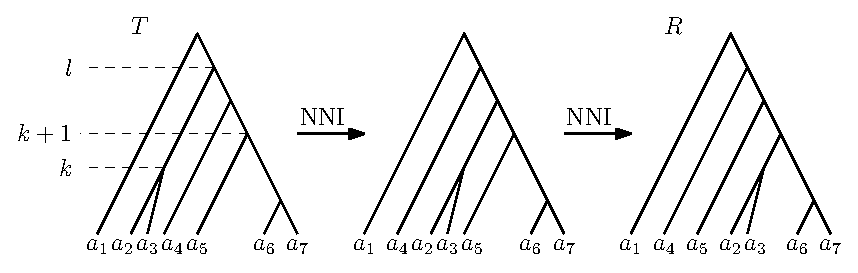
\includegraphics[width=0.8\textwidth]{nni_path_caterpillar.eps}
		\caption{Example of a tree $T$ with two rank intervals and a sequence of $\nni$ moves that results in a tree $R$ with one rank interval as described in the proof of Lemma~\ref{lemma:nni_path_to_caterpillar}.}
		\label{fig:nni_path_caterpillar}
	\end{figure}
\end{proof}

With this lemma we are able to prove that the diameter of $\rnni(\infty)$ is quadratic in $n$.
\begin{corollary}
	The diameter of $\rnni(\infty)$ is less or equal to $3 \frac{(n-1)(n-2)}{2}$.
\end{corollary}

\begin{proof}
	Let $T$ and $R$ be two trees in $\rnni(\infty)$.
	With Lemma~\ref{lemma:nni_path_to_caterpillar} we know that any tree can be connected to a caterpillar tree by a sequence of $\nni$ moves.
	Moreover, the proof of the lemma implicitly proposes an algorithm to convert a tree into a caterpillar tree by removing rank intervals by a top-down approach.
	We show that the paths from a tree to a caterpillar tree that are given by this algorithm have at most length $\frac{(n-1)(n-1)}{2}$.
	Since we also know that the set of caterpillar trees is convex in $\rnni$ (Theorem~\ref{thm:caterpillar_convex_rnni}), and hence the maximum distance between caterpillar trees is bounded by the diameter $\frac{(n-1)(n-2)}{2}$ of $\rnni$ (Corollary~\ref{cor:diameter_rnni}), this corollary follows.

	For finding the maximum length of a path computed by the algorithm suggested in the proof of Lemma~\ref{lemma:nni_path_to_caterpillar}, we consider every iteration (induction step).
	In each of these, at least one rank interval turns into an edge.
	The number of $\nni$ moves needed for this depends on the rank of the upper node bounding the rank interval.
	If we assume the worst case, that is, every interval except for the edge $[(T)_{n-1},(T)_{n-2}]$ is a rank interval, then there are $i$ $\nni$ moves needed in iteration $i$.
	Since there are $n-2$ iterations, it follows that at most $\frac{(n-1)(n-2)}{2}$ $\nni$ moves are needed to get from an arbitrary tree to a caterpillar tree.
	\todo{I suspect writing the algorithm down properly and using it to prove Lemma~\ref{lemma:nni_path_to_caterpillar} and this corollary might be easier than this. This explanation of the 'implicitly' defined algorithm is not sufficient.}
\end{proof}

\summary{Radius of $\rnni$ is equal to its diameter.}
For proving that the radius of $\rnni$, which is defined $\min\limits_{\text{tree } T}\max\limits_{\text{tree }R} d(T,R)$, equals its diameter, we need the following lemma.
\todo{Can we come up with a more intuitive description of what the radius of a graph is?}

\begin{lemma}
	For every tree on $n$ leaves exists a caterpillar tree with distance $\frac{(n-1)(n-2)}{2}$ from it in $\rnni$.
	\label{lemma:max_dist_ctree}
\end{lemma}

\begin{proof}
	We prove this lemma by induction on the number of leaves $n$.
	The base case $n=3$ is trivial, as all three trees in this space are caterpillar trees with distance one.
	For the induction step we consider an arbitrary tree $T$ with $n + 1$ leaves.
	Let $T'$ be the tree on $n$ leaves resulting from deleting one of the cherry leaves, which we denote by $x$, of $T$.
	By applying the induction hypothesis on $T'$ we can find a caterpillar tree $R'$ that has distance $\frac{(n-1)(n-2)}{2}$ to $T'$.
	Now consider the tree $R$ resulting from adding the leaf $x$ at the top of $R'$ such that the root of $R$ has $x$ and $R'$ as children.

	In the first iteration of $\findpath$ the leaf $x$ moves down by $\nni$ moves until it reaches the second cherry leaf $y$ of $T$ and builds a cherry with it, which then is moved down by rank swaps as depicted in Figure~\ref{fig:max_dist_ctree}.
	There are $n-1$ $\rnni$ moves needed for this as $(x,y)_R$ moves down from the root with rank $n$ to the cherry of rank one.
	The tree at the end of this first iteration on $\fp(T,R)$ is equals $R'$ when ignoring the leaf $x$ and its parent.
	Since the cluster $\{x,y\}$ is not considered again in $\findpath$, the remaining part of $\fp(T,R)$ contains the same moves as $\fp(T',R')$ from which we can follow that $|\fp(T,R)| = |\fp(T',R')| + n-1$.
	\todo{Is it OK to phrase it like this?}
	Therefore it is $d(T,R) = \frac{(n-1)(n-2)}{2} + n-1 = \frac{n(n-1)}{2}$, which proves the lemma.
	\begin{figure}[ht]
		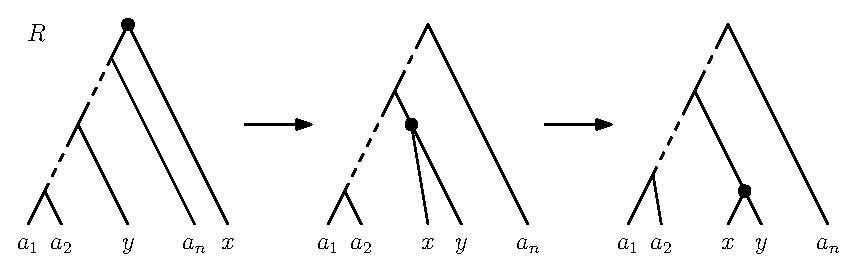
\includegraphics[width=0.8\textwidth]{max_dist_ctree.eps}
		\caption{Initial $n - 1$ $\rnni$ moves of $\fp(R,T)$ as described in the proof of Lemma~\ref{lemma:max_dist_ctree}.
		Removing the leaf $x$ and suppressing the non-root node of degree two from the tree on the right results in $R'$ as described in the lemma.}
		\label{fig:max_dist_ctree}
	\end{figure}
\end{proof}

\begin{proposition}
	The radius of the $\rnni$ graph equals its diameter, i.e. $\rad(\rnni) = \frac{(n-1)(n-2)}{2}$.
\end{proposition}

\begin{proof}
	From Lemma~\ref{lemma:max_dist_ctree} we know that there is a tree with distance $\frac{(n-1)(n-2)}{2}$ from any given tree.
	Hence the radius equals the diameter of $\rnni$.
\end{proof}

\subsection{Cluster Property}

\summary{Definition of Cluster Property and why it is relevant.}

\summary{$\rnni$ has the cluster property.}
\begin{theorem}
	The $\rnni$ graph has the cluster property.
\end{theorem}


\section{$\rnni(\rho)$}

\todo{How can we connect $\rnni(\rho)$ to $\dtt$?}

\subsection{Caterpillar Trees}

\summary{The set of caterpillar trees is convex in $\rnni(\rho)$ for $\rho > 1$.}
\begin{corollary}
	The set of caterpillar trees is convex in $\rnni(\rho)$ if and ony if $\rho \geq 1$.
\end{corollary}

\begin{proof}
	We start with proving that if the set of caterpillar trees is convex, then it is $\rho \geq 1$.
	More specifically, we show that if $\rho < 1$, then the set of caterpillar trees is not convex, from which the previous statement follows.
	Therefore we consider the following example of trees with four leaves.
	Let
	\begin{align*}
		T &= [\{1,2\},\{1,2,3\},\{1,2,3,4\}]\text{ and }\\
		R &= [\{3,4\},\{1,3,4\},\{1,2,3,4\}].
	\end{align*}
	The shortest among all caterpillar paths between $T$ and $R$ has length three and is depicted at the bottom of Figure~\ref{fig:caterpillar_non_convex}.
	However, there is a path that is shorter than this path and has length $2 + \rho$, which is smaller than three for $\rho < 1$.
	This path is depicted at the top of Figure~\ref{fig:caterpillar_non_convex}.
	Hence, the set of caterpillar trees is not convex if $\rho < 1$.
	\begin{figure}[ht]
		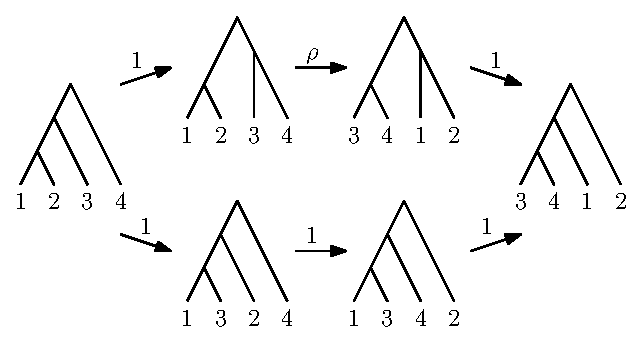
\includegraphics[width=0.5\textwidth]{caterpillar_non_convex.eps}
		\caption{A shortest caterpillar path between caterpillar trees $T$ and $R$ at the bottom and a path consisting of non-caterpillar trees at the top.
		The path at the top is shorter than the one at the bottom for all $\rho<1$.}
		\label{fig:caterpillar_non_convex}
	\end{figure}

	It remains to prove that if $\rho \geq 1$, then the set of caterpillar trees is convex.
	With Theorem~\ref{thm:caterpillar_convex_rnni} we know that this is true for $\rho = 1$.
	Moreover, the statement for $\rho > 1$ follows from the same theorem as described in the following, where we assume that $\rho > 1$.
	All paths between any two trees in $\rnni(\rho)$ are longer or have equal length to the path containing the same moves in $\rnni$, as the weights of the moves in $\rnni(\rho)$ are greater or equal to the weights of the same moves in $\rnni$.
	Specifically, the only paths that have the same length in $\rnni$ and $\rnni(\rho)$ are paths that contain only $\nni$ moves.
	It follows that caterpillar paths of $\rnni$ have the same length in $\rnni(\rho)$, while other paths might be longer in $\rnni(\rho)$, but cannot be shorter than the same path in $\rnni$.s
	And as there is a shortest caterpillar path between all caterpillar trees in $\rnni$, this path is shortest path in $\rnni(\rho)$ as well.
	This proves that the set of caterpillar trees is convex in $\rnni(\rho)$ for $\rho \geq 1$, which completes the proof.
\end{proof}

\subsection{Diameter and Radius}

\summary{Diameter for $\rnni(0)$ follows from $\nni$}
Not only for $\rnni$, but also for $\rnni(0)$, we know the diameter from previous results.
As rank moves in $\rnni(0)$ weigh zero, the distance between two trees in this space is the same as the $\nni$ distance between these trees when ignoring ranks.
Therefore, these graphs have the same diameter.

\begin{proposition}
	The diameter of $\rnni(0)$ is $\Theta(n \log(n))$.
	\label{prop:diameter_nni}
\end{proposition}

\begin{proof}
	This follows from the diameter of the $\nni$ graph, which is known \autocite{Semple2003-nj} to be $\Theta(n \log(n))$.
\end{proof}

\summary{Results for $\rnni$ and $\rnni(0)$ give us bounds for the diameters of all spaces with $0 < \rho < 1$.}
With the previous results in Corollary~\ref{cor:diameter_rnni} and Proposition~\ref{prop:diameter_nni} we can infer bounds for diameters of spaces $\rnni(\rho)$ with $0 < \rho < 1$.
A path in $\rnni(\rho)$ between two trees corresponds to paths in $\rnni(0)$ and $\rnni(1)$ that contain the same moves, but have different total length, due to the different weighing of rank moves.
Therefore, the length of such a path is bounded from below by the length of the corresponding path in $\rnni(0)$ and from above by the corresponding path in $\rnni(1)$.
With Corollary~\ref{cor:diameter_rnni} and Proposition~\ref{prop:diameter_nni} it follows that the diameter of $\rnni(\rho)$ with $\rho < 1$ is bounded from below by $\Theta(n \log(n))$ and from above by $\frac{(n-1)(n-2)}{2}$.

\summary{Diameter of $\rnni(\rho)$ for $\rho > 1$.}
So far $\rnni(\rho)$ for $0 \leq \rho \leq 1$ has been the centre of our investigation of diameters.
We now continue by considering spaces $\rnni(\rho)$ for $\rho > 1$, where rank moves are more expensive than $\nni$ moves.
Specifically, we give an upper bound for the diameter of $\rnni(\infty)$ from which we can follow that all spaces $\rnni(\rho)$ have a diameter less or equal to this bound.
Before this, however, we need to observe that for $\rnni(\infty)$ every pair of trees is connected by a path consisting of $\nni$ moves only.

\summary{Radius of $\rnni(\rho)$ for other values of $\rho$.}

\subsection{Cluster Property}

\summary{$\rnni(0)$ does not have cluster property.}
\begin{proposition}
	$\rnni(0)$ does not have the cluster property.
\end{proposition}

\summary{Cluster Property of $\rnni(\rho)$ for $\rho \neq 0, 1$?}


%TODO: Leave this as a section or do we want a section (not just subsection) for DtT?
\section{Generalisation}

\summary{All (?) results from $\rnni$ transfer to discrete time-trees.}

\summary{How partition lattices correspond to $\rnni$.}

\summary{Implementation of FP}

\todo{We should mention that in an implementatino of $\findpath$ on discrete time-trees we would not add leaves but implement length moves, to save memory}

\end{document}